\documentclass{article}
\usepackage{graphicx}

\title{Artificial Intelligence \\ WHPP Project Report}
\date{2019-04-19}
\author{Kallinteris Andreas\\ Orfanoudakis Stavros}

\begin{document}
\maketitle
\section*{Introduction}
This report analyzes our implementation of a standard genetic algorithm to solve the WHPP problem (according to the specification) where for genomes are the work shifts of the employees.
The following sections show how each step of the algorithm was implemented.
\section*{Population Initialize}
The initial population is feasible.
\section*{Crossbreeding}
Due to the limitations of hard constraint (number of people working per shift) the option of crossbreeding all of the population together is not possible,
instead we breed 2 schedules a large amount of times,
out of the two schedules that are selected for breeding the one is the best and the other is a random one with $p_sel$ to select a different one in each iteration (doing anything smarter/more complex increases the runtime of the program by a huge amount).
\section*{Mutation}
Due to the limitations of hard constraint (number of people working per shift) mutating the schedules is quite limited (we can't mutate per genome).
Mutating the schedules is done by randomly switching 2 shifts of workers and evaluating the difference.
\section*{Terminating Conditions}
At first a simple iteration counter $iter_{max}$ was used to terminate the top level loop but it was observed that after a small number of iteration the algorithm stopped improving (due to reaching a local maxima),
therefore to combat this after a certain number of iterations $iter_{imr}$ without any improvement the algorithm exits.

\section*{Performance Tuning-Testing}

Below we are gonna represent few graphs about different ways of crossover and mutation while changing the values of the according probabilities. In every graph will be displayed the best person of the population and the average of the current generation. The y-axis is indicating the total score, greater score means more soft constraints are satisfied. The x-axis is displaying the number of iterations.

\subsection*{a)}

\begin{table}[!htb]
\centering
\begin{tabular}{|c|c|c|c|c|}
\hline
\textbf{Pcross} & \textbf{Pmut} & \textbf{Psel} & \textbf{Mutation Function} & \textbf{Pop} \\ \hline
60\% & 1\% & 50\% & random daily & 256 \\ \hline
\end{tabular}
\end{table}
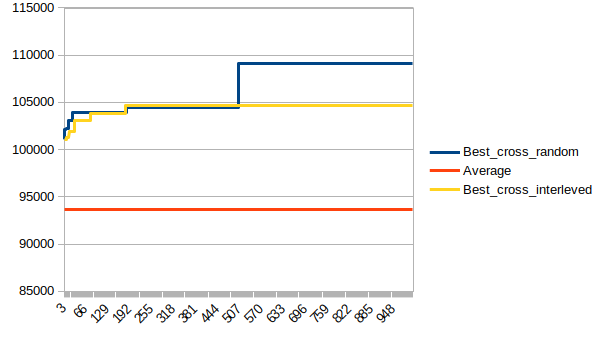
\includegraphics[scale=0.75]{11}

\subsection*{b)}
\begin{table}[!htb]
\centering
\begin{tabular}{|c|c|c|c|c|}
\hline
\textbf{Pcross} & \textbf{Pmut} & \textbf{Psel} & \textbf{Mutation Function} & \textbf{Pop} \\ \hline
60\% & 1\% & 50\% & random reverse & 256 \\ \hline
\end{tabular}
\end{table}
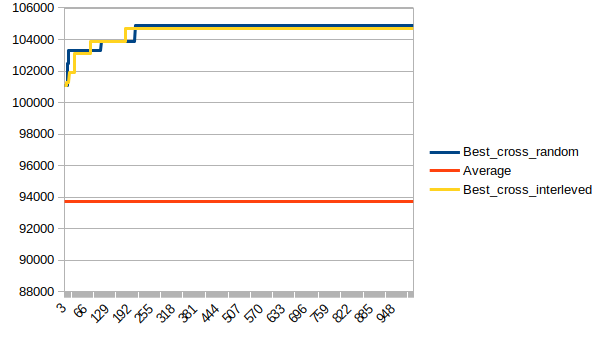
\includegraphics[scale=0.75]{12}

\subsection*{c)}
\begin{table}[!htb]
\centering
\begin{tabular}{|c|c|c|c|c|}
\hline
\textbf{Pcross} & \textbf{Pmut} & \textbf{Psel} & \textbf{Mutation Function} & \textbf{Pop} \\ \hline
60\% & 1\% & 50\% & random reverse & 256 \\ \hline
\end{tabular}
\end{table}
In this case we are using \textbf{elitism} in selection section, so it tends to a local maximum much faster

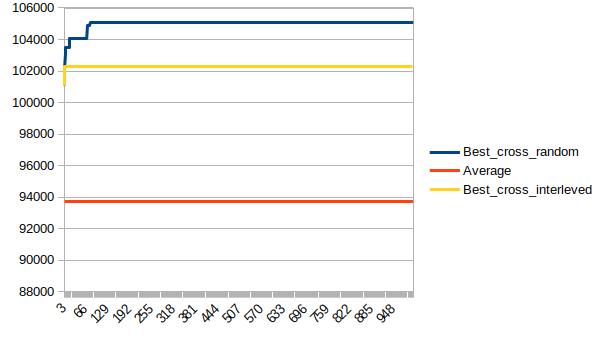
\includegraphics[scale=0.75]{13}

\subsection*{d)}
\begin{table}[!htb]
\centering
\begin{tabular}{|c|c|c|c|c|}
\hline
\textbf{Pcross} & \textbf{Pmut} & \textbf{Psel} & \textbf{Mutation Function} & \textbf{Pop} \\ \hline
60\% & 1\% & 50\% & random reverse & 100 \\ \hline
\end{tabular}
\end{table}
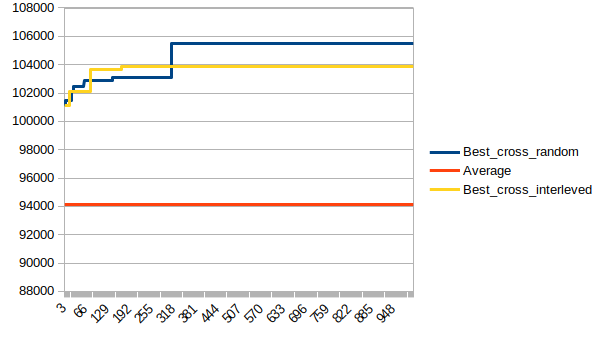
\includegraphics[scale=0.75]{14}

\subsection*{f)}
\begin{table}[!htb]
\centering
\begin{tabular}{|c|c|c|c|c|}
\hline
\textbf{Pcross} & \textbf{Pmut} & \textbf{Psel} & \textbf{Mutation Function} & \textbf{Pop} \\ \hline
10\% & 1\% & 100\% & random daily & 256 \\ \hline
\end{tabular}
\end{table}
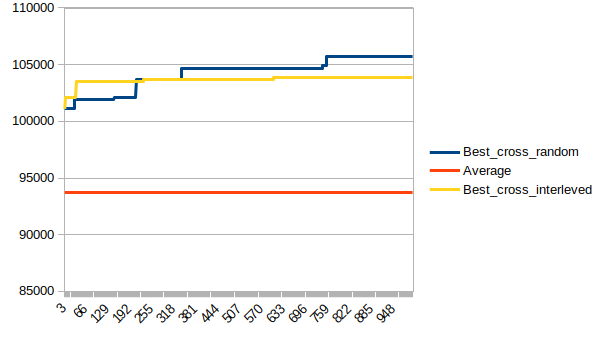
\includegraphics[scale=0.75]{16}

\subsection*{g)}
\begin{table}[!htb]
\centering
\begin{tabular}{|c|c|c|c|c|}
\hline
\textbf{Pcross} & \textbf{Pmut} & \textbf{Psel} & \textbf{Mutation Function} & \textbf{Pop} \\ \hline
10\% & 1\% & 100\% & random reverse & 256 \\ \hline
\end{tabular}
\end{table}

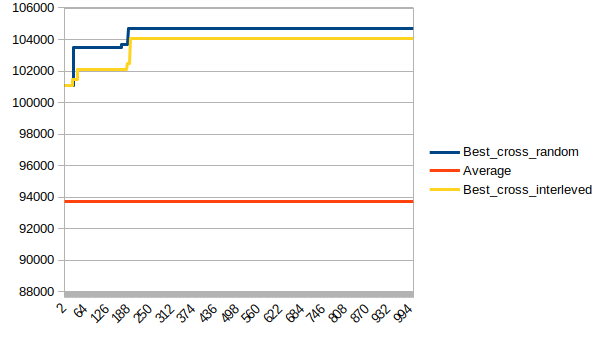
\includegraphics[scale=0.75]{17}

 A lot more different combinations where tested but these where representing the various aspects of our algorithm the best.\\

$iter_{max}$ was set to a very high value as the algorithm is always terminated by $iter_{imr}$ (note: if we had a time deadline $iter_{max}$ is set accordingly),
$iter_{imr}$ was set to 256 as higher values never produced better results,
the population count scales the performance of the algorithm from 4 to 16000 sub linearly any increase past 256 very increases the and does scale any further are 16000 (16k has the same performance as 32k and 64k),
$p_{mut}$ was set to 1 as any lower values resulted in lower performance
$p_{cross}$ did not have any effect on the performance of the algorithm but lower values increased the runtime of the program,
$p_{sel}$ does not affect the performance in any measurable way.
\section*{Conclusion}
The performance of the genetic algorithm produces similar results to naively generating a ton of random schedules and selecting the best one when taking in account total runtime expect when the runtime is really limited.
An option of for improving the performance of the genetic algorithm would be to improve the selection but that would come with further degradation to the runtime.
The best overall performance can be obtained by running many small/simple genetic algorithms and getting the best result rather that having few complex ones (when taking into account runtime) because with a small amount of computational power we can reach a local minimum.
\end{document}